\documentclass{./../../Latex/teaching_slides}

\usepackage{venndiagram}
\usepackage{tikz}
\usepackage{pgfplots}
\usetikzlibrary{arrows.meta}

\begin{document}

\title{ECON 441 \\ \vspace{0.4em} \normalsize Introduction to Mathematical Economics}
\author{Div Bhagia}
\date{Lecture 10 \\ Constrained Optimization}

%%%%%%%%%%%%%%
\begin{frame}[noframenumbering, plain]
\maketitle
\end{frame}

%%%%%%%%%%%%%%
\begin{frame}{Utility Maximization}
Maximize:
$$ f(x_1, x_2) = x_1 x_2  $$ \\~\\

Subject to the budget constraint:
$$ 2x_1 + x_2 = 40 $$ \\~\\
 
To find $x_1^*$ and $x_2^*$, we could substitute $x_2=40-2x_1$ and use our first-order and second-order conditions.
\end{frame}

%%%%%%%%%%%%%%
\begin{frame}{Utility Maximization}
\vspace{-1.5em}
$$ f(x_1, x_2) = x_1 (40-2x_1)=40x_1-2x_1^2  $$ \\~\\
 
\begin{tikzpicture}[remember picture,overlay]
    \draw[gray!50, opacity=0.75] (0,-4.5) grid[step=0.75] (14.25,0.75);
  \end{tikzpicture}
\end{frame}

%%%%%%%%%%%%%%
\begin{frame}{Constrained Maximization}
Substitution doesn't always work, get's complicated with many variables and constraints. \\~\\

Thankfully, we have the method of Lagrange multiplier. \\~\\
Lagrange function:
$$ L(x_1, x_2, \lambda) = x_1 x_2 + \lambda(40-2x_1-x_2) $$

$\lambda$ is the Lagrange multiplier.  \\~\\

Now apply FOC for the case of 3 variables ($x_1, x_2, \lambda)$. 
\end{frame}

%%%%%%%%%%%%%%
\begin{frame}{Utility Maximization}
$$ L(x_1, x_2, \lambda) = x_1 x_2 + \lambda(40-2x_1-x_2) $$ \\~\\

First-order conditions:
\begin{align*}
\frac{\partial L}{\partial x_1} &= x_2-2 \lambda = 0 \\ 
\frac{\partial L}{\partial x_2} &= x_1- \lambda = 0 \\ 
\frac{\partial L}{\partial \lambda} &= 40-2x_1-x_2 = 0 
\end{align*}
\end{frame}

%%%%%%%%%%%%%%
\begin{frame}{Lagrange-Multiplier Method}
Given an objective function
$$
y=f(x_1, x_2)
$$
subject to the constraint
$$
g(x_1, x_2)=c
$$
where $c$ is a constant. We can write the Lagrange function as
$$
L(x_1,x_2,\lambda)=f(x_1, x_2)+\lambda[c-g(x_1, x_2)]
$$
\end{frame}

%%%%%%%%%%%%%%
\begin{frame}{Lagrange-Multiplier Method}
$$
L(x_1,x_2,\lambda)=f(x_1, x_2)+\lambda[c-g(x_1, x_2)]
$$ \\~\\
First-order conditions:
\begin{align*}
\frac{\partial L}{\partial x_1} &= f_1(x_1^*, x_2^*)- \lambda^* \cdot g_1(x_1^*, x_2^*) = 0 \\ 
\frac{\partial L}{\partial x_2} &= f_2(x_1^*, x_2^*)- \lambda^* \cdot g_2(x_1^*, x_2^*) = 0 \\ 
\frac{\partial L}{\partial \lambda} &= c-g(x_1^*, x_2^*) = 0 
\end{align*}
\end{frame}

%%%%%%%%%%%%%%
\begin{frame}{Utility Maximization}
\begin{columns}[T]
\begin{column}{0.7\textwidth}
  	\centering \vspace{0.5em}
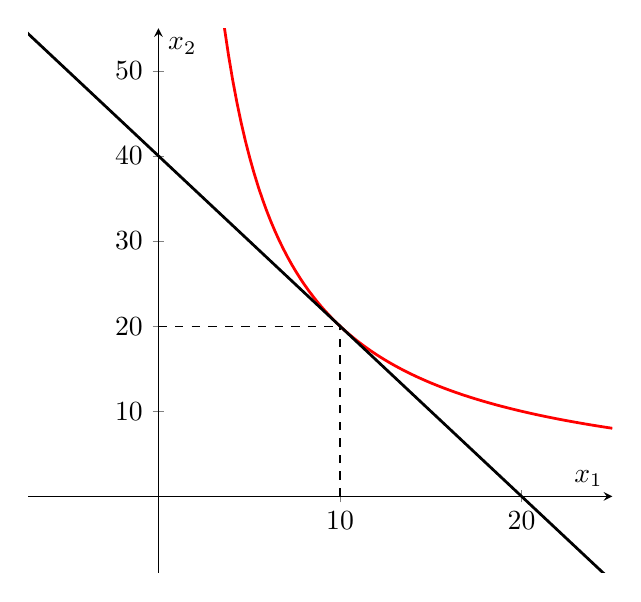
\begin{tikzpicture}
\begin{axis}[ymin=-9, ymax=55, xmax=25, axis lines = center, 
	xlabel = \(x_1\), ylabel = {\(x_2\)},ytick distance=10, xtick distance=10, width=9cm, height=8.5cm]
% Utility function
\addplot [domain=2:25, samples=100, color=red,line width=1,]{200*x^(-1)};
% Budget line
\addplot [domain=-10:25, samples=100, color=black, line width=1,]{40-2*x};
% Dashed lines
\draw[dashed] (axis cs:10,0) -- (axis cs:10,20);
\draw[dashed] (axis cs:0,20) -- (axis cs:10,20);
\end{axis}
\end{tikzpicture}
\end{column}	
\begin{column}{0.4\textwidth}
At the optimal point:
$$ \frac{\partial f / \partial x_1}{\partial f / \partial x_2} = \frac{\partial g / \partial x_1}{\partial g / \partial x_2}$$ \\~\\
Balance trade-off: \\ optimize $f$ vs satisfy $g$
\end{column}	
\end{columns}
\end{frame}

%%%%%%%%%%%%%%
\begin{frame}{Interpretation of the Lagrange Multiplier}
At the optimum:
$$
L(x^*_1,x^*_2,\lambda^*)=f(x^*_1, x^*_2)+\lambda^*[c-g(x^*_1, x^*_2)]
$$
What if $c$ changes by a little bit? \pause
\begin{align*}
\frac{dL^*}{dc} &=f_1 \cdot \frac{d x_1^*}{dc}+ f_2 \cdot \frac{d x_2^*}{dc} + \lambda^*\left[ 1- g_1 \cdot \frac{d x_1^*}{dc}- g_1 \cdot \frac{d x_1^*}{dc} \right] \\ 
& = \underbrace{(f_1-\lambda^* \cdot g_1)}_{0} \cdot \frac{d x_1^*}{dc} + \underbrace{(f_2-\lambda^* \cdot g_2)}_{0} \cdot \frac{d x_2^*}{dc} + \lambda^* = \lambda^*
\end{align*}
\end{frame}

%%%%%%%%%%%%%%
\begin{frame}{Utility Maximization}
$$ L(x_1, x_2, \lambda) = x_1 x_2 + \lambda(40-2x_1-x_2) $$ \\~\\

At the optimum: 
$$x_2* = 2 x_1^*, \quad 2x_1^* + x_2^* = 40 \quad \rightarrow \quad x_1^*=10, x_2^*=20, \lambda^* = 10$$

If my income increases by \$1, by how much does my utility increase? $\lambda^* = 10$
\end{frame}


%%%%%%%%%%%%%%
\begin{frame}{Example I}
\vspace{-2em}
$$ \max_{\{x_1,x_2\}} \quad x_1^2x_2 \quad s.t. \quad 2x_1^2 + x_2^2 = 3$$
 \begin{tikzpicture}[remember picture,overlay]
    \draw[gray!50, opacity=0.75] (0,-5.25) grid[step=0.75] (14.25,0);
  \end{tikzpicture}
\end{frame}

%%%%%%%%%%%%%%
\begin{frame}{Example II}
\vspace{-2em}
$$ \max_{\{x,y\}} \quad x^a y^b \quad s.t. \quad x+y=10$$
 \begin{tikzpicture}[remember picture,overlay]
    \draw[gray!50, opacity=0.75] (0,-5.25) grid[step=0.75] (14.25,0);
  \end{tikzpicture}
\end{frame}

%%%%%%%%%%%%%%
\begin{frame}{Example III}
\vspace{-1.5em}
$$ \max_{\{x_1,x_2\}} \quad x_1^{1/3} x_2^{2/3} \quad s.t. \quad x_1 + 4 x_2 = 30 $$
 \begin{tikzpicture}[remember picture,overlay]
    \draw[gray!50, opacity=0.75] (0,-5.25) grid[step=0.75] (14.25,0);
  \end{tikzpicture}
\end{frame}

%%%%%%%%%%%%%%
\begin{frame}{More Generally}
\vspace{-1.5em}
$$ \max_{\{x_1,x_2\}} \quad x_1^{\alpha} x_2^{\beta} \quad s.t. \quad p_1 x_1 + p_2 x_2 = m $$
 \begin{tikzpicture}[remember picture,overlay]
    \draw[gray!50, opacity=0.75] (0,-5.25) grid[step=0.75] (14.25,0);
  \end{tikzpicture}
\end{frame}

%%%%%%%%%%%%%%
\begin{frame}{Multiple Variables}
Objective function:
$$ \text{Maximize } f\left(x_{1}, x_{2}, \cdots, x_{n}\right) \quad \text{subject to} \quad g\left(x_{1}, x_{2}, \cdots, x_{n}\right)=c 
$$
Lagrange function:
$$
L=f\left(x_{1}, x_{2}, \cdots, x_{n}\right)+\lambda\left[c-g\left(x_{1}, x_{2}, \cdots, x_{n}\right)\right]
$$
First-order conditions:
$$
\begin{aligned}
&L_{i}=f_{i}\left(x_{1}, x_{2}, \cdots, x_{n}\right)-\lambda g_{i}\left(x_{1}, x_{2}, \cdots, x_{n}\right) \quad[i=1,2, \cdots, n] \\
&L_{\lambda}=c-g\left(x_{1}, x_{2}, \cdots, x_{n}\right) 
\end{aligned}
$$
\end{frame}

%%%%%%%%%%%%%%
\begin{frame}{Multiple Constraints}
Maximize $f\left(x_{1}, x_{2}, \cdots, x_{n}\right)$, subject to 
$$
g\left(x_{1}, x_{2}, \cdots, x_{n}\right)=c \quad \text{and} \quad h\left(x_{1}, x_{2}, \cdots, x_{n}\right)=d
$$
Lagrange function:
$$
L=f\left(x_{1}, x_{2}, \cdots, x_{n}\right)+\lambda\left[c-g\left(x_{1}, x_{2}, \cdots, x_{n}\right)\right]+\mu\left[d-h\left(x_{1}, x_{2}, \cdots, x_{n}\right)\right]
$$
First-order conditions:
$$
\begin{aligned}
&L_{\lambda}=c-g\left(x_{1}, x_{2}, \cdots, x_{n}\right)=0 \\
&L_{\mu}=d-h\left(x_{1}, x_{2}, \cdots, x_{n}\right)=0 \\
&L_{i}=f_{i}\left(x_{1}, x_{2}, \cdots, x_{n}\right)-\lambda g_{i}\left(x_{1}, x_{2}, \cdots, x_{n}\right)-\mu h_{i}\left(x_{1}, x_{2}, \cdots, x_{n}\right)=0 
\end{aligned}
$$
\end{frame}

%%%%%%%%%%%%%%
\begin{frame}{Example IV}
\vspace{-2em}
$$ \max_{\{x,y,z\}} \quad yz + xz \quad s.t. \quad y^2+z^2=1 \quad and \quad  xz=3 $$
 \begin{tikzpicture}[remember picture,overlay]
    \draw[gray!50, opacity=0.75] (0,-5.25) grid[step=0.75] (14.25,0);
  \end{tikzpicture}
\end{frame}

%%%%%%%%%%%%%%%%%%%%
\begin{frame}{Intertemporal Utility Maximization}
\vspace{-1.25em}
$$ 	U = U(c_1, c_2) =  \ln c_1 + \beta \ln c_2 \quad \quad 0<\beta<1$$
\vspace{-0.65em}

\begin{witemize}
  \item $y_1,y_2>0$: income in period 1 and 2
  \item Income you save $s$ in period 1 earns interest $r>0$
  \item In which case,
 $$ c_1 + s = y_1 \quad \quad \quad  c_2 = y_2 + (1+r) s $$
 \item Combining these constraints:
$$ c_1 + \frac{1}{1+r} c_2 = \underbrace{y_1 + \frac{1}{1+r} y_2}_{m \equiv \text{present-discounted income}}$$
%$$ m = y_1 + \frac{1}{1+r} y_2 $$}} $$
\end{witemize}
\end{frame}

%%%%%%%%%%%%%%%%%%%%
\begin{frame}{Intertemporal Utility Maximization}
\vspace{-1.5em}
$$ \max_{\{c_1,c_2\}} \quad U(c_1, c_2) = \ln c_1 + \beta \ln c_2 \quad s.t. \quad c_1 + \frac{1}{1+r} c_2 = m $$
 \begin{tikzpicture}[remember picture,overlay]
    \draw[gray!50, opacity=0.75] (0,-5.25) grid[step=0.75] (14.25,0);
  \end{tikzpicture}
\end{frame}


%%%%%%%%%%%%%%
\begin{frame}{References and Homework Problems}
	\begin{witemize}
  \item References for today: Sections 12.1 and 12.2
  \item Homework: Exercise 12.2: Questions 1--4 + Examples from today's class
\end{witemize}
\end{frame}


\end{document}